\documentclass[12pt]{article}
\usepackage{amsmath,amsfonts,times}
\usepackage{graphicx,color,tikz,pgfplots}
\usepackage[paperwidth=8.1cm,paperheight=6.1cm,lmargin=0in,rmargin=0in,tmargin=0.in,bmargin=0.in]{geometry}
\usepackage{bm}
\usetikzlibrary{arrows,shadings,shapes.arrows,decorations.pathreplacing,calc, positioning}
\usepgfplotslibrary{fillbetween}

\begin{document}
\centering
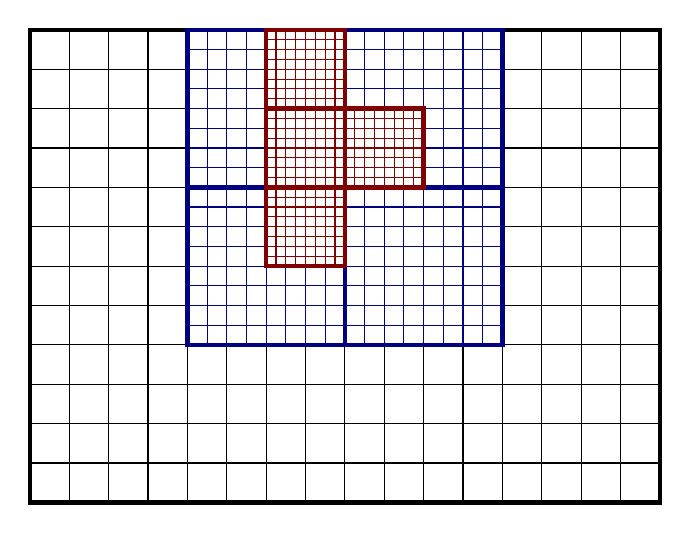
\begin{tikzpicture}[on grid]

  % Parent grid
  \draw[step=5mm, black, thin] (0,0) grid  (8,6); %defining grids
  \draw[black,ultra thick] (0,0) rectangle (8,6);%marking borders

  % LEVEL 1 GRIDS
  \draw[step=2.5mm, blue!50!black, thin] (2,2) grid (4,4);  %Nested grid 1
  \draw[blue!50!black, ultra thick] (2,2) rectangle (4,4);%marking borders
  
  \draw[step=2.5mm, blue!50!black, thin] (2,4) grid (4,6);  %Nested grid 2
  \draw[blue!50!black, ultra thick] (2,4) rectangle (4,6);%marking borders
  
  \draw[step=2.5mm, blue!50!black, thin] (4,4) grid (6,6);  %Nested grid 3
  \draw[blue!50!black, ultra thick] (4,4) rectangle (6,6);%marking borders
  
  \draw[step=2.5mm, blue!50!black, thin] (4,2) grid (6,4);  %Nested grid 4
  \draw[blue!50!black, ultra thick] (4,2) rectangle (6,4);%marking borders


  % LEVEL 2 GRIDS
  \draw[step=1.25mm, red!50!black, thin] (3,3) grid (4,6);  %Nested grid 1
  \draw[red!50!black, ultra thick] (3,3) rectangle (4,4);%marking borders
  \draw[red!50!black, ultra thick] (3,4) rectangle (4,5);%marking borders
  \draw[red!50!black, ultra thick] (3,5) rectangle (4,6);%marking borders

  \draw[step=1.25mm, red!50!black, thin] (4,4) grid (5,5);  %Nested grid 1
  \draw[red!50!black, ultra thick] (4,4) rectangle (5,5);%marking borders

%%   \draw[step=5mm, red!50!black, thin] (8.0,6.0) grid (10,8);  %Nested grid 1
%%   \draw[red!50!black, ultra thick] (8.0,6.0) rectangle (10,8);%marking borders

%%   \draw[step=5mm, red!50!black, thin] (6.0,8.0) grid (8,10);  %Nested grid 1
%%   \draw[red!50!black, ultra thick] (6.0,6.0) rectangle (8,10);%marking borders

%%   \draw[step=5mm, red!50!black, thin] (8.0,8.0) grid (10,10);  %Nested grid 1
%%   \draw[red!50!black, ultra thick] (8.0,8.0) rectangle (10,10);%marking borders

%%   \draw[step=5mm, red!50!black, thin] (10.0,8.0) grid (12,10);  %Nested grid 1
%%   \draw[red!50!black, ultra thick] (10.0,8.0) rectangle (12,10);%marking borders

%%   \draw[step=5mm, red!50!black, thin] (12.0,8.0) grid (14,10);  %Nested grid 1
%%   \draw[red!50!black, ultra thick] (12,8.0) rectangle (14,10);%marking borders

%%   \clip(0,0) rectangle (8,8);
%% %  \draw[black, ultra thick, draw=black, fill=green!50!black, fill opacity=0.5] (8.0,0.0) circle (4.5cm);
\end{tikzpicture}

\end{document} 
